\chapter{Implementation}

This chapter deals with the description of implementing and modifying the LCS.

For this thesis there was created a test project in the Infomedia TFS where I could do my work. This was so that I would not mess up Infomedia's inflow while trying to make the algorithms work correctly.

\section{Basic Implementation}
First off the Cosine algorithm was implemented in said test project, and then the basic implementation of LCS was implemented.

Then the basic LCS algorithm was implemented in the project, to be used for further development.

\lstset{style=sharpc}
\begin{lstlisting}[caption=Basic LCS implementation in C$^\sharp$, captionpos=b]

public int LongestCommonSubstring(string str1,
	 string str2)
{
    if (String.IsNullOrEmpty(str1) 
    	|| String.IsNullOrEmpty(str2))
    return 0;
	
	int[,] num = new int[str1.Length, str2.Length];
	int maxlen = 0;

    for (int i = 0; i < str1.Length; i++)
  	{
    	for (int j = 0; j < str2.Length; j++)
        {
        	if (str1[i] != str2[j])
            	num[i, j] = 0;
            else
            {
            	if ((i == 0) || (j == 0))
                	num[i, j] = 1;
                else
                    num[i, j] = 1 + num[i - 1, j - 1];

                    if (num[i, j] > maxlen)
                    {
                    	maxlen = num[i, j];
                  	}
           	}
     	}
	}
    return maxlen;
}

\end{lstlisting}

The LCS works by taking in two strings as arguments and then comparing them character by character (see figure ~\ref{LcsExplained}. This works really well for finding substrings that can have been obfuscated in long lines of text. How ever in this thesis, the main objective is to find substrings of plain words rather than finding bits and pieces.

When comparing two articles with the LCS, the algorithm finds a lot of substrings, but only keeps the longest by default
\begin{figure}
	\centering
	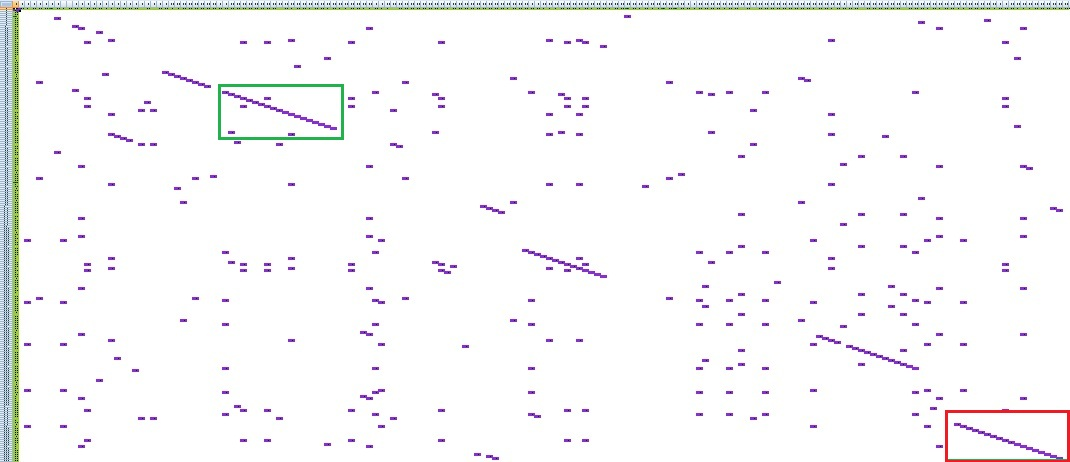
\includegraphics[scale=0.4]{figures/LcsExample}
	\caption{Diagram showing the result of two article being compared by using LCS, and plotted in Excels. See Appendix A.1 for bigger image. The green and red boxes indicates longest common substrings found.}
	\label{LcsEx}
\end{figure}

The green rows seen in Figure ~\ref{LcsEx} is an article (one article along the topmost edge of the y-axis and one along leftmost edge of the x-axis) split into words (in the basic implementation the articles would be split in characters as seen in figure 3.4 ~\ref{LcsExplained}, this figure is from the updated version of LCS). All the purple boxes indicates where a match has been found, a diagonal line indicates a row (substring) of matches. The longest one would be the \textit{'Longest Common Substring'} and the length of that would be returned by the algorithm. In the example from Figure ~\ref{LcsEx} there are two substrings of equal length (each having a length of 19 words (in the basic LCS the length would the number of characters, including white spaces)), how ever as LCS only returns the length of a single longest common substring (the longest found) and the second one (marked in the red box) is same length, LCS returns the length of the first (marked in the green box) substring. Again, as this example is made out of words rather than characters, the result could vary in case of counting actual characters, but for demonstration purposes the figure explains the idea.

In the case of a perfect match (require both articles to be of the exact same length). A line along the diagonal will be drawn.

\begin{figure}
	\centering
	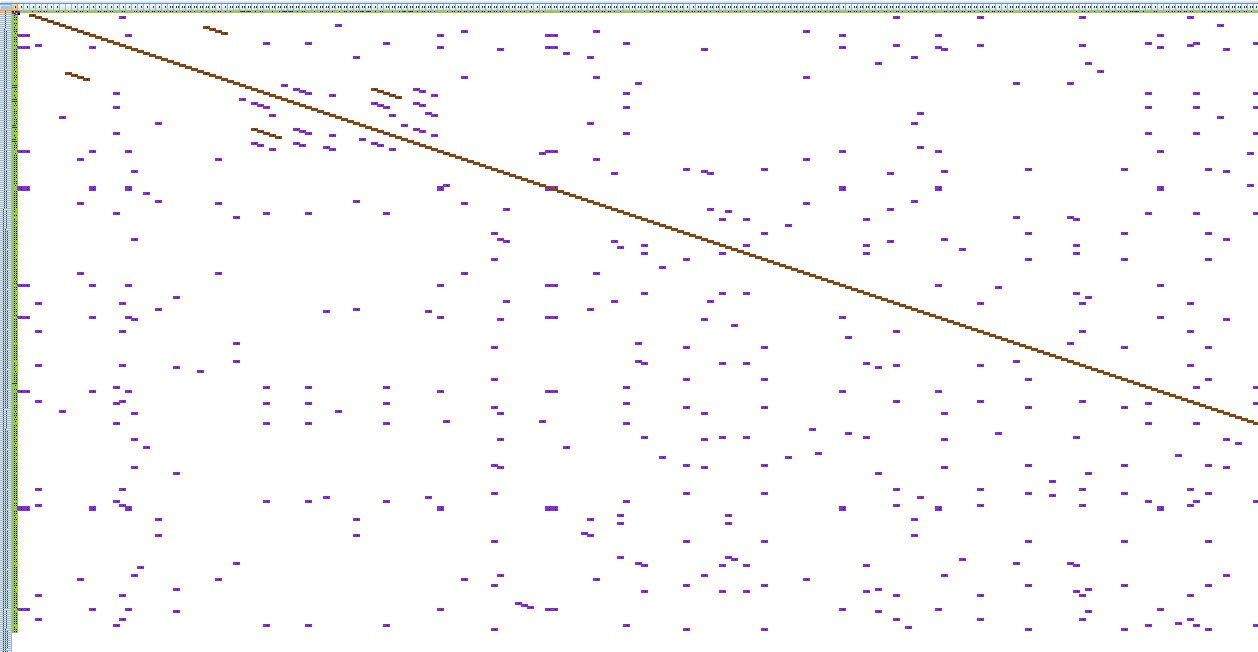
\includegraphics[scale=0.35]{figures/PerfectMatch}
	\caption{Diagram showing a part of an almost perfect match (the article along the y-axis is slightly longer than the article along the x-axis). The long brown diagonal line indicates the longest common substring found.}
	\label{Match}
\end{figure}

In Figure ~\ref{Match} there is two article that are almost 100\% identical. One of the articles ~\cite{JV1} is slightly shorter than the other article ~\cite{Lemvig1}. The on line content of the second article is protected by a payment wall, the article content can be found in Appendix B ~\ref{Levmig1:text}.

The next step was to modify the LCS algorithm to make suit the needs of this thesis. When looking at article duplicates, it makes more sense to look for entire words rather than single characters. This is because when an article is duplicated, any obfuscation or alteration would be done by cutting out sections of the article or moving sections around or adding new sections.

\section{Modification of LCS - String Comparison}
As hinted both in the text of the last section and also in figure ~\ref{LcsEx}, the next step was to modify LCS to compare whole words (string) instead of single letters (char). There are of course pros and cons to this approach. One of the pros would be that we could improve the performance of the algorithm. If we assume that the average word length is roughly five characters long\footnote{\url{http://www.wolframalpha.com/input/?i=average+english+word+length} - although it is for English words, it is most likely not that different from Danish.}, that means that comparing articles on a character by character basis increases the number of comparisons by a factor of 25 as compared to doing it word by word. This will therefore mean we can get a rather big performance boost, and when talking about an inflow that just for my test corpus contains ~22800 articles, but can be as many as 40000 articles daily, this factor will make quite the impact. Another pro is that we are looking for word duplication, not for sentences obfuscated within other sentences, therefore we do not really need to look at single characters.

On the cons side is the fact that if we are looking for words rather than single characters the algorithm becomes more prone to spelling errors. If the word \textit{'doomsday device'} was included in an article and in an article that is a duplicate of that article was a spelling error \textit{'doomday device'}, this would cause the character based substring to be slightly longer than than the words based substring. The character based substring would return \textit{'sday device'} whereas the word based substring would only contain \textit{'device'}. This can be an issue within texts that have \underline{many} spelling error, but that case is highly unlikely to appear in articles this thesis is dealing with, as one would assume that journalists are pretty okay with correct spelling. 

So even though modifying LCS to compare words with words rather than characters, can return incorrect results, the likely hood of this being a substantial error source is negligible.

\subsection{Issue With Word (String) Comparisons}
The issue with comparing words rather than single characters in data science, is that the way comparison is done with data types, which is not as easy as when a human would do text comparison. For a human, reading and comparing two list of single letters, would be substantially slower than comparing two lists of words. This is based on how we recognize both single letters and words. A computer does things in a completely different way.\\* The basic implementation of LCS compares chars with chars, a char being a basic data type in most modern objective oriented programming languages (Java, C$^\sharp$, Objective C). Comparing primitives is a simple operation, just checking their values. The modification being implemented would compares Strings with Strings, a String being a data type \textit{'object'} in object oriented languages. A String is internally a list of chars, that makes up the whole String, so comparing a String object with another String object is basically doing a char comparison (with some minor differences, such as String comparison also checks the length of the Strings).

However, in a future implementation of the modified version of LCS, one could transform the Strings into an int (one could use the word map generated by the Cosine algorithm for this), so that each word gets it's own int value, comparing the words as int values would be much faster than both the String and char comparison. This is because an int is a primitive, like the char, and instead of having to check a lot of chars for each "word", there would only be a need to check a single int value for each word. This would improve the overall performance of LCS dramatically (approximately by a factor 25, by applying the same theory as above, each word on average being five characters long) as the list of words (int) would be substantially shorter than the lists of chars. 

Due to the fact that I did not contemplate this until late in the work process, there have been no time to implement a String to int conversion in the LCS modification.

For testing purposes it is nicer and easier to read text split up into words rather than text split in chars, so that is a bonus of the string comparison modification of LCS.

So even though it adds no immediate performance boost, this is both a step on the way and helping hand in terms of evaluating the results from LCS.

\section{Collection of Substrings}
Another modification to the LCS that would help finding article duplicates would be to make LCS create a collection of substrings. The benefits of this would to some extend help eliminate the error prone ways of LCS. If looking at two articles that would be considered a perfect match (same length, same article text), except for the word in middle of the text in of the articles. If this have been changed, misspelled or forgotten, this would cause the basic implementation of LCS to return that the length of the longest common substring would be ~50\% of the article's length. How ever, if we create a collection of substring we can in part work around this issue. Then we would find two substrings, one before the middle word (that is missing or in other way not present in the same form as in the other article) and one after the middle word. Our combination of substrings would then return a length that is close to 100\% of the article length.

When doing this modification one should consider using a threshold that indicates the minimum length a substring should have in order to be included. As seen in both figure ~\ref{LcsEx} and ~\ref{Match} there is a lot of single word matches found when LCS is traversing the article texts. So an effective threshold would be one that filters away the noise, but it not so high that important (in terms of finding duplicates) sentences are filtered out. For this thesis the threshold have been set to four, meaning that all substrings consisting of four or more words are being stored as a result.

When creating the collection of substrings their lengths will be added and compared to the total length, thus creating a hopefully more correct image of whether two articles match or not.

\lstset{style=sharpc}
\begin{lstlisting}[caption=Modified version of LCS, captionpos=b]

public Dictionary<String, String>
 LongestCommonSubstring(List<String> str1,
  List<String> str2, int threshold)
    {
	  if (str1.Count == 0 || str2.Count == 0)
	      throw new Exception
	      ("One or both documents was empty.");

      int[,] num = new int[str1.Count, str2.Count];

      var combined = new Dictionary<string, string>();

      for (int i = 0; i < str1.Count; i++)
      {
         for (int j = 0; j < str2.Count; j++)
         {
            if (str1[i] != str2[j])
                num[i, j] = 0;
            else
            {
              if ((i == 0) || (j == 0))
                  num[i, j] = 1;
              else
                  num[i, j] = 1 + num[i - 1, j - 1];

              if (num[i, j] >= threshold)
              {
                // Find the start index 
                // of the current substring
                String index = 
                ((i - num[i, j]) + 
                ", " + (j - num[i, j]));

                String insert = "";
                // Do we already have this key stored?
                if (!combined.ContainsKey(index))
                {
                    var words = new List<String>();
                    for (int x = 3; x > 0; x--)
                    {
                       words.Add(str1[i - x]);
                    }
                    foreach (String word in words)
                       insert += word + " ";
                    insert += str1[i] + " ";
                    combined.Add(index, insert);
                }
                else
                {
                    String valueStore = combined[index];
                    valueStore += str1[i] + " ";
                    combined[index] = valueStore;
                }
              }
            }
          }
        }
       return combined;
   }

\end{lstlisting}



As seen in figure ~\ref{SubstringsEx} the addition of substring collection significantly alters the result from what we would have seen, had we only been using the basic LCS implementation. Judging from this diagram the two articles obviously have a lot in common. To tell if the article really have something in common it is needed to take a look at their semantic content. This can be done by using semantic algorithms\footnote{\url{http://en.wikipedia.org/wiki/Semantic_matching}}, which is something that could be a part of a future implementation of this project, but it is not implemented in this thesis. Another way of doing this is by reading it the old fashion way, with your own eyes.  All of the verification done in a prototype is expected to be done this way, once the users are satisfied that no or only very few errors would bypass the algorithms, then the verification would be left to the algorithms (as per figure ~\ref{Architecture}). 


\begin{figure}
	\centering
	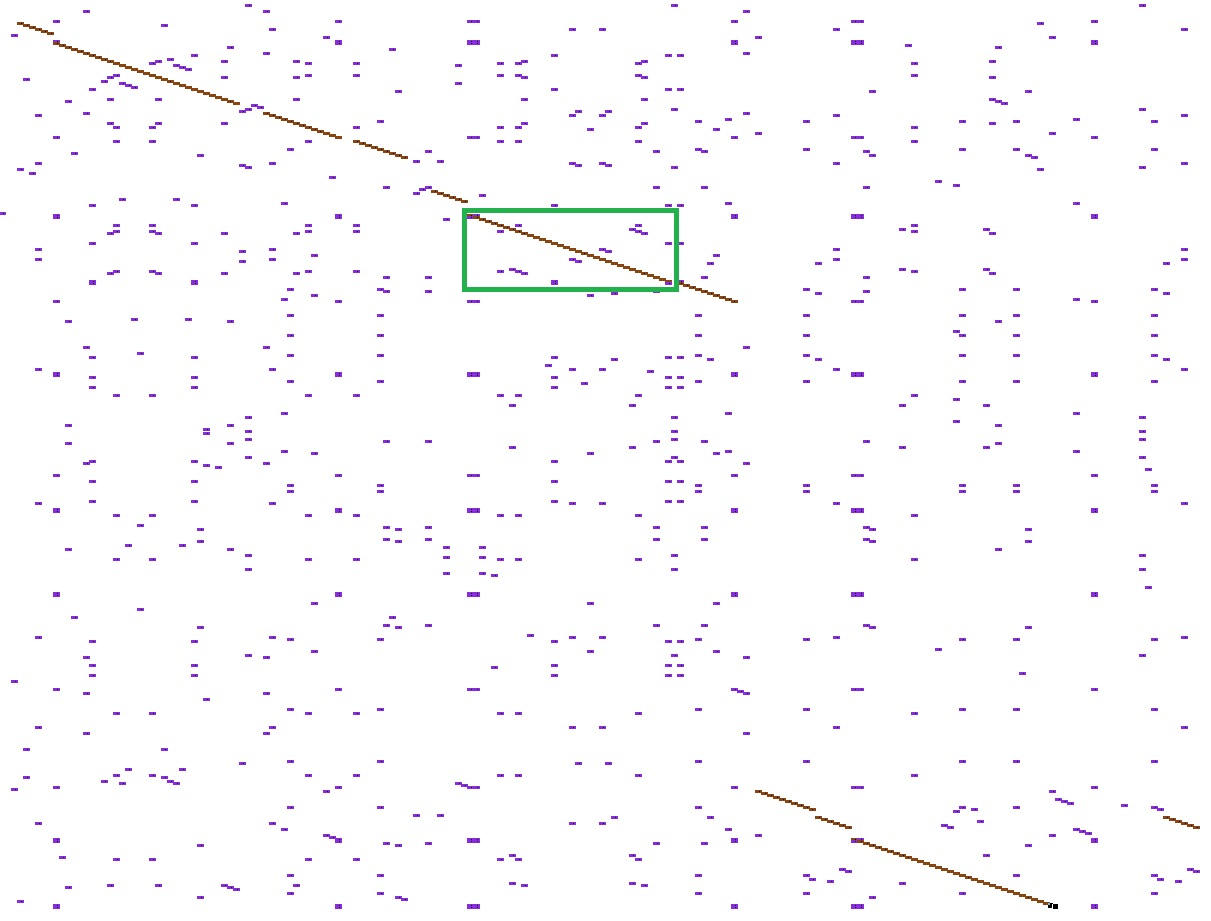
\includegraphics[scale=0.35]{figures/SubstringCollection}
	\caption{The result of having a collection of substrings. All the brown lines indicates where a substring with the minimum length of four have been found. If only the longest substring had been returned as the result, only the substring (marked by the brown line) in the green box would have been returned.}
	\label{SubstringsEx}
\end{figure}





